\documentclass[12pt,a4paper]{article}
\usepackage[utf8]{inputenc}
\usepackage[spanish]{babel}
\usepackage{amsmath}
\usepackage{amsfonts}
\usepackage{amssymb}
\usepackage{graphicx}
\usepackage[left=2cm,right=2cm,top=2cm,bottom=2cm]{geometry}

%--------------------------------------------------------%
% Paquetes usados sólo para esta relación de ejercicios  %
%--------------------------------------------------------%

\usepackage{enumitem}
\usepackage{algorithm}
\usepackage{algorithmic}
\usepackage[hidelinks]{hyperref}

\usepackage{subcaption}


\author{Ignacio Aguilera Martos}
\title{Práctica 3 \\ Visión por Computador}
\date{22 de Diciembre de 2018}

\setlength{\parindent}{0cm}


\begin{document}
	\maketitle

	\tableofcontents

	\newpage

	%p 56

%	\framebox[16cm][c]{\LaTeX}

\section{Ejercicio 1}

Emparejamiento de descriptores.
\begin{itemize}
  \item Mirar las imágenes en imagenesIR.rar y elegir parejas de imágenes que tengan partes de escena comunes. Haciendo uso de una máscara binaria o de las funciones extractRegion() y clickAndDraw(), seleccionar una región en la primera imagen que esté presente en la segunda imagen. Para ello sólo hay que fijar los vértices de un polígono que contenga a la región.
  \item Extraiga los puntos SIFT contenidos en la región seleccionada de la primera imagen y calcule las correspondencias con todos los puntos SIFT de la segunda imagen (ayuda: use el concepto de máscara con el parámetro mask)
  \item Pinte las correspondencias encontradas sobre las imágenes.
  \item Jugar con distintas parejas de imágenes, valorar las correspondencias correctas obtenidas y extraer conclusiones respecto a la utilidad de esta aproximación de recuperación de regiones/objetos de interés a partir de descriptores de una región.
\end{itemize}

\subsection*{\underline{Solución}}

Las parejas que he escogido han sido dos para ejemplificar el buen comportamiento cuando las imágenes son similares entre sí y otra en la que el reconocimiento no es tan bueno.

\vspace{10px}

Las parejas escogidas son:

\begin{figure}[H]
  \centering
    \begin{subfigure}{0.45\textwidth}
      
\includegraphics[scale=0.33]{./Imagenes/1.png}
    \end{subfigure}
    \begin{subfigure}{0.45\textwidth}
      
\includegraphics[scale=0.33]{./Imagenes/4.png}
    \end{subfigure}
    \caption{Imágenes 1 y 4}
\end{figure}

\begin{figure}[H]
  \centering
    \begin{subfigure}{0.45\textwidth}
      
\includegraphics[scale=0.33]{./Imagenes/23.png}
    \end{subfigure}
    \begin{subfigure}{0.45\textwidth}
      
\includegraphics[scale=0.33]{./Imagenes/24.png}
    \end{subfigure}
    \caption{Imágenes 23 y 24}
\end{figure}

\begin{figure}[H]
  \centering
    \begin{subfigure}{0.45\textwidth}
      
\includegraphics[scale=0.33]{./Imagenes/91.png}
    \end{subfigure}
    \begin{subfigure}{0.45\textwidth}
      
\includegraphics[scale=0.33]{./Imagenes/92.png}
    \end{subfigure}
    \caption{Imágenes 91 y 92}
\end{figure}

La forma de proceder es, mostrar la imagen para que se pueda seleccionar la región de la misma que se desee. Esta región es diferenciada del resto mediante una máscara. La construcción de dicha máscara se hace tomando los puntos que determinan el polígono de la región y, mediante la función fillConvexPoly se rellena esta área a blanco, esto es $(255,255,255)$. Tras esto sólo tenemos que crear una matriz de ceros del mismo tamaño que la imagen y, en dichos puntos poner el valor 1. Con esto tendríamos una máscara que podemos aplicar a la función detectAndCompute para hallar los keypoints y descriptores sólo de la región que engloba el polígono.

\vspace{10px}

Hay que tener en cuenta que la detección puede ser buena si realmente hay un parecido importante entre la región que hemos seleccionado y alguna región de la imagen con la que queremos emparejar. Por ejemplo veamos los dos primeros ejemplos y analicémoslos.

\begin{figure}[H]
  \centering
  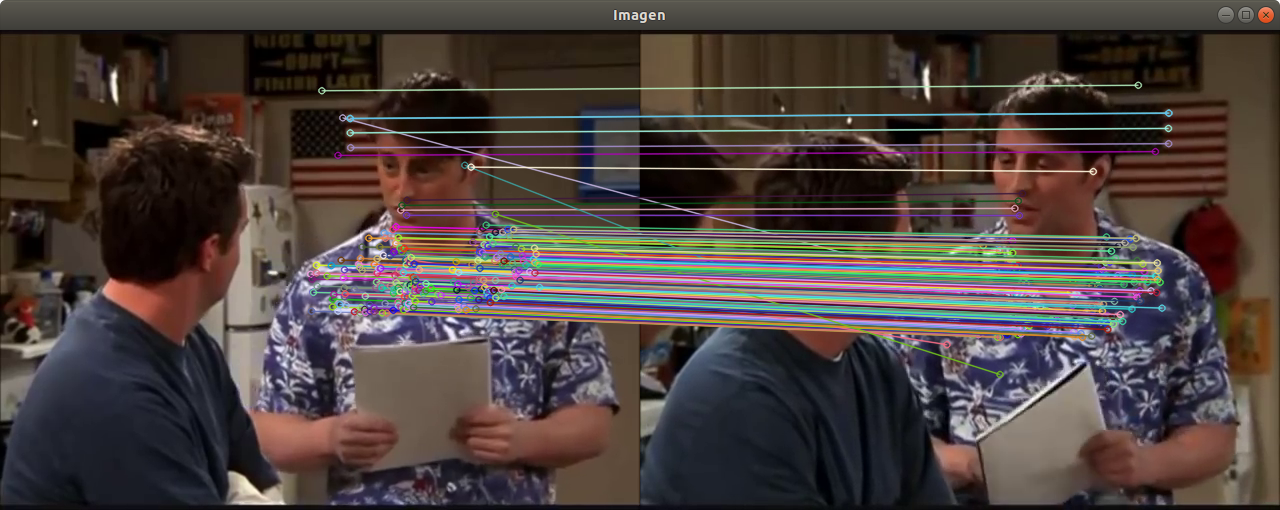
\includegraphics[scale=0.35]{./Imagenes/Ejercicio1-1.png}
  \caption{Emparejamiento con las imágenes 91 y 92}
\end{figure}

\begin{figure}[H]
  \centering
  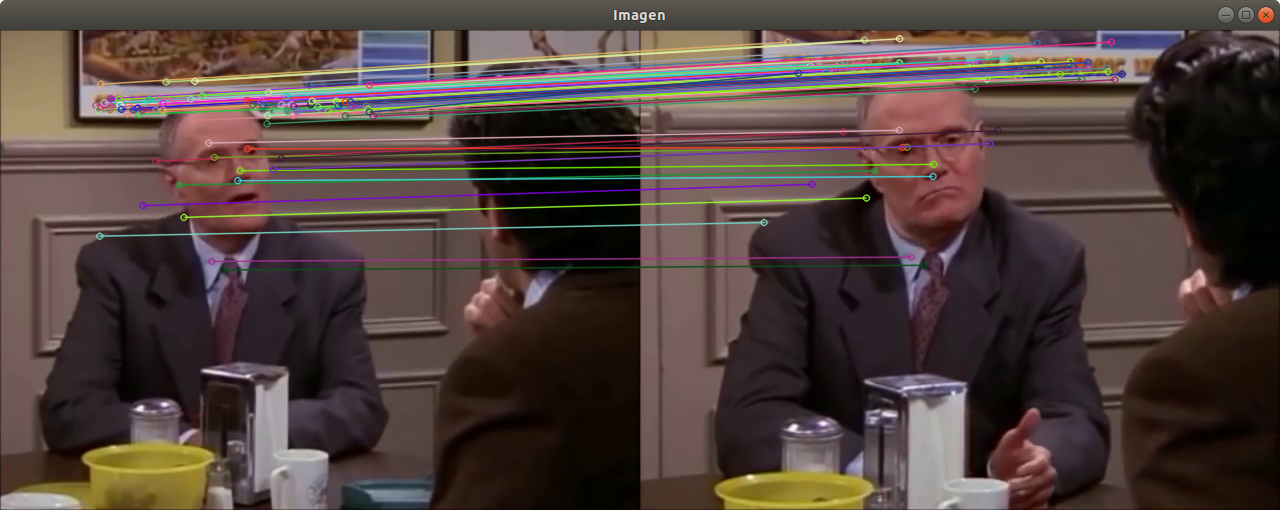
\includegraphics[scale=0.35]{./Imagenes/Ejercicio1-2.png}
  \caption{Emparejamiento con las imágenes 23 y 24}
\end{figure}

Como podemos ver claramente en estas dos imágenes el emparejamiento es muy bueno puesto que los parecidos entre las dos es muy alto. Es prácticamente la misma cara con la misma escena y el mismo fondo, por lo que no sólo se empareja la cara o la figura de la persona, si no, también el fondo como en el segundo de los casos con el cuadro que se encuentra tras la persona.

\vspace{10px}

Cabe decir que esta detección puede variar enormemente como en el siguiente caso paradigmático.

\begin{figure}[H]
  \centering
  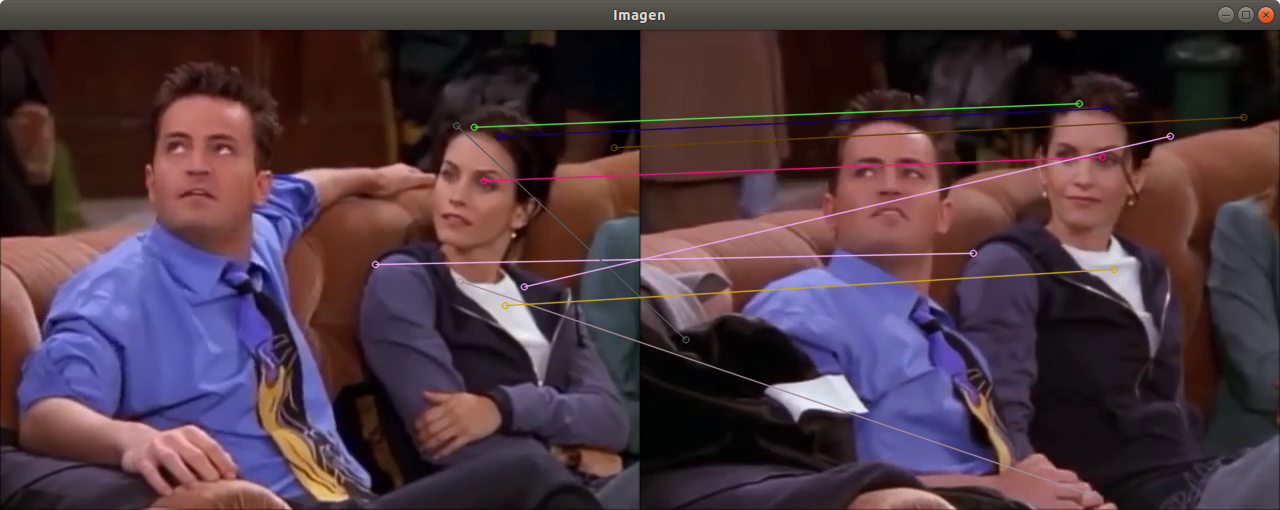
\includegraphics[scale=0.35]{./Imagenes/Ejercicio1-3.png}
  \caption{Emparejamiento con las imágenes 1 y 4}
\end{figure}

En este caso podemos ver que la detección es mucho peor pero analicemos por qué. Realmente si observamos cada uno de los keypoints como se relacionan con la imagen de la derecha vemos que el emparejamiento de los mismos es razonable salvo dos de ellos, pero este emparejamiento es muy pobre porque no hemos obtenido suficientes puntos de interés en la región como para obtener un emparejamiento sólido como en los dos primeros casos.

\vspace{10px}

Ahora bien, podemos tomar también dos imágenes de una escena que compartan una figura como por ejemplo la mujer que se enseña en las imágenes siguientes:

\begin{figure}[H]
  \centering
    \begin{subfigure}{0.45\textwidth}
      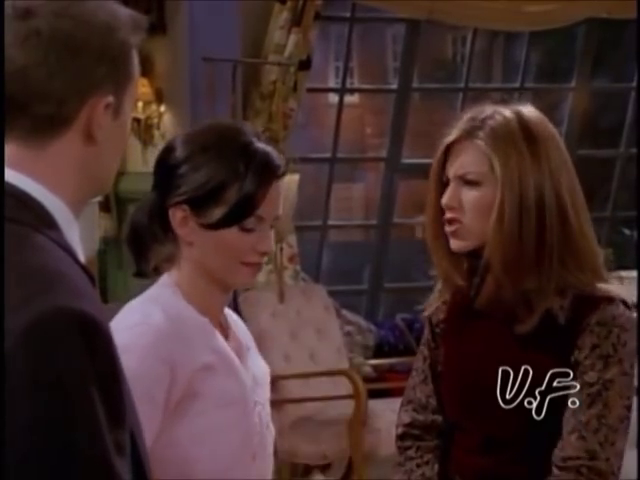
\includegraphics[scale=0.33]{./Imagenes/142.png}
    \end{subfigure}
    \begin{subfigure}{0.45\textwidth}
      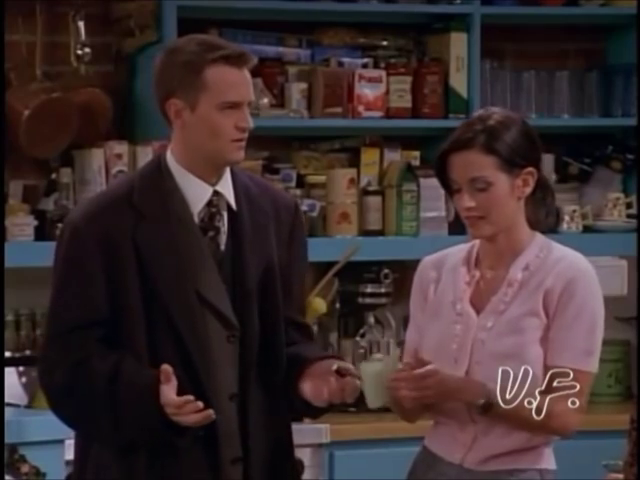
\includegraphics[scale=0.33]{./Imagenes/143.png}
    \end{subfigure}
    \caption{Imágenes 142 y 143}
\end{figure}

Veamos que la detección en este caso no es satisfactoria cuando tomamos el polígono sobre la figura de la mujer.

\begin{figure}[H]
  \centering
  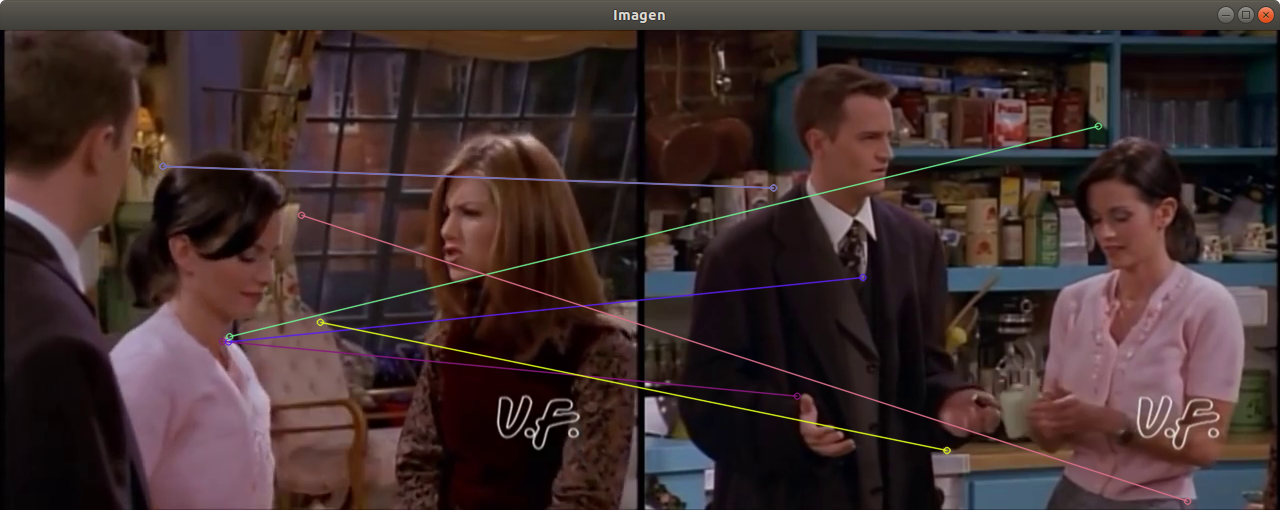
\includegraphics[scale=0.35]{./Imagenes/Ejercicio1-4.png}
  \caption{Emparejamiento con las imágenes 142 y 143}
\end{figure}

Como podemos observar nosotros estamos viendo que la mujer que aparece en la imagen de la izquierda es la misma que en la parte de la derecha pero la detección asigna los puntos de forma completamente errónea con respecto a la figura de la misma. Este fallo viene sobre todo dado porque el fondo de las imágenes es completamente distinto y por tanto, los puntos de interés tomados (que hacen el contraste en este caso de la mujer con el fondo) se ven completamente irrelevantes con respecto a la correlación que hace de los mismos.

\vspace{10px}

Por lo tanto podemos concluir que el uso de esta aproximación a la recuperación de regiones de interés a partir de descriptores de una región es en general útil pero conociendo las limitaciones, tanto de la obtención de un número de puntos de interés demasiado bajo como de el emparejamiento erróneo que pueda realizar la misma con otra imagen en la que sí comparten una región pero el fondo o la iluminación han cambiado y no se perciben las regiones como similares.

\end{document}
